\documentclass{article}
\author{Alejandro Zubiri}
\date{Tue Dec 03 2024}
\title{Sobre la precisión}

\usepackage{amsmath, amsfonts, amsthm, graphicx}
\graphicspath{{../images/}}

\newtheorem{definition}{Definición}

\begin{document}
\maketitle
\begin{definition}[Precisión]
    Definimos la precisión como la proximidad entre las medidas de una misma muestra.
\end{definition}
    A la hora de saber cómo de preciso es un estimador, necesitamos conocer alguna propiedad de este que
    indique la proximidad entre sus datos, y para esto tenemos la \textbf{varianza}. Precisamente, gracias
    a la varianza (o a la desviación típica, que es la raíz de esta) podemos conocer la dispersión 
    entre los datos. Cuanto más dispersos los datos, más varianza. Y precisamente por esto,
    se define la precisión de un estimador $\hat{\theta }$ como:
    \begin{equation}
        \begin{split}
            \text{precisión }(\hat{\theta }) = \frac{1}{var(\hat{\theta })}
        \end{split}
    \end{equation}
    Esta es precisamente la definición usada en el libro "Fundamentos de estadística" de Daniel Peña, página
    283:
    \begin{center}
        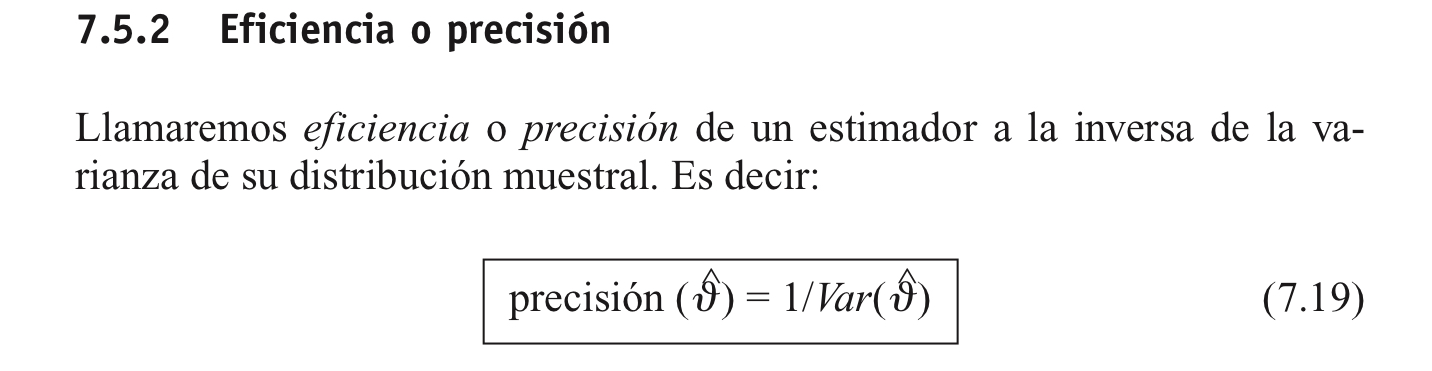
\includegraphics[scale=0.25]{20241203_164517000_iOS.jpg}
    \end{center}
    Sin embargo, en clase se nos dijo que se mide la precisión mediante el \textbf{error de muestreo}:
    \begin{equation}
        \begin{split}
            e(\hat{\theta }) = \frac{\sigma }{\sqrt{n}}
        \end{split}
    \end{equation}
    Esta definición sigue la misma lógica (en función de la desviación típica del estimador) solo que un
    mayor error de muestreo indica una menor precisión y viceversa.\\
    Ambas definiciones, pese a que diferentes, aportan la misma información a la hora de indicar qué
    estimador es más preciso, por eso considero que usar cualquiera de las dos definiciones es correcto
    a la hora de determinar la precisión, y creo que restringir el uso de una única medida
    (solo porque sea la que se ha enseñado en clase) sería castigar la comprensión y habilidad del
    examinado a la hora de resolver el problema.
\end{document}